\thispagestyle{empty}
\spacing{1.5}

\begin{wrapfigure}{r}{0.25\textwidth}
	\scalebox{0.5}{
		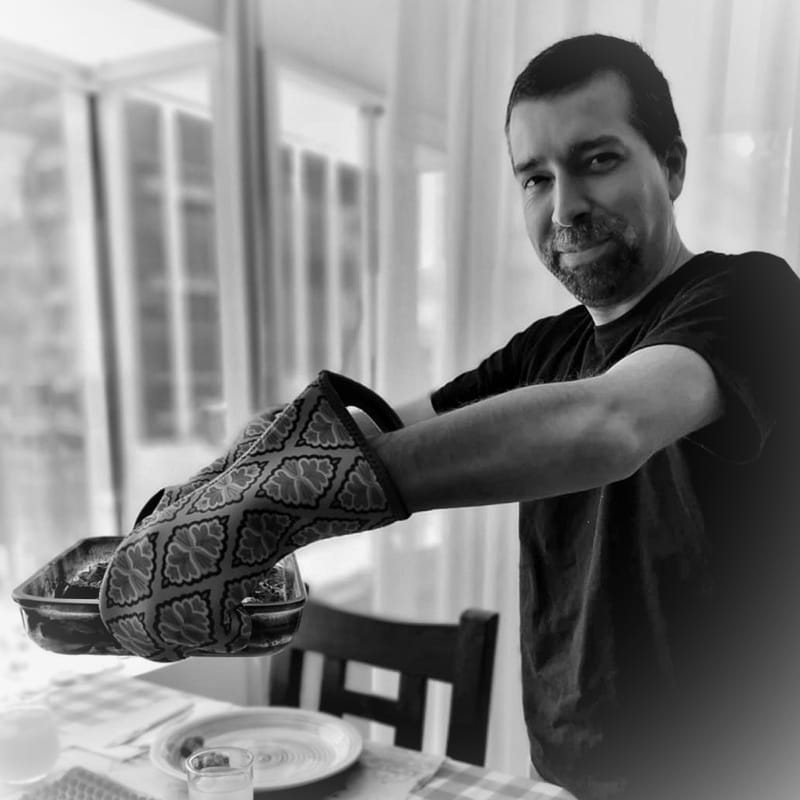
\includegraphics[width=0.48\textwidth]{autor}
	}
\end{wrapfigure} 

Este libro es un pequeño tributo a la memoria de las recetas de cocina de la familia, al sabor, al disfrute de los alimentos pero más que todo eso a la compañía o reunión de familia, amigos y seres queridos, que alguno de ellos
ya no están. 

En la vida cotidiana, de pequeños hemos visto a alguno de nuestros padres que dedican tiempo en la cocina y realizan algunos platos que más que alguna ocasión han sido el deleite nuestro como hijos. En ocasiones, habían desayunos, almuerzos o comidas que en sí eran especiales, eran diferentes del menú diario por algún tipo de evento, otras en cambio, eran comidas que quizás en algún momento no queríamos como niños, pero que ahora como adulto, apreciamos el detalle, el contexto, y cada uno de esos platos puede evocar un hermoso recuerdo.

A lo largo de la vida, las recetas se han transmitido de generación en generación por diversos medios, algunos han tenido la dicha de aprender directamente de sus familiares, otros en cambio por el echo de mirar a otros, y otros simplemente al comer, y ver los elementos en la comida, y comenzar con esa curiosidad de cómo es que conforman el plato en sí. 

No quiero extenderme mucho más pues esto no es un estudio científico o algún tipo de documento de análisis,  simplemente es una recopilación de las recetas típicas del hogar en el que viví, así como también algunas otras que he aprendido a lo largo de la vida, recetas tradicionales chilenas, alguna cosa extranjera, y que son relativamente fáciles de hacer en casa.

Porque en la vida, en ocasiones, es grato darse tiempo a uno mismo en compañía con los suyos, y qué mejor momento que en un almuerzo, una once, una cena, o incluso un desayuno, y compartir momentos, vivencias que nos llenarán el alma y nuestros recuerdos para nuestras memorias en la vejez...
